\section{模型评估与选择}
\subsection{经验误差与拟合}
\myitem 错误率:m个样本中有a个样本分类错误,则错误率$E=a/m$.
\myitem 精度:$1-a/m$
\myitem 误差:学习器的实际预测输出与样本的真实输出之间的差异;训练集上的叫\underline{训练误差}/\underline{经验误差},新样本上的叫\underline{泛化误差};
\myitem 过拟合(更容易遇到的情况):将个例的特殊性错误地视为样本的普遍性;欠拟合:没有学好.
\par 过拟合无法避免(N=NP问题尚未证明),只能缓解或减小其风险
\myitem 模型选择:在多种学习算法中,选择合适的算法中的合适的参数配置.
\subsection{评估方法}
\myitem 测试集测试学习器对新样本的判断力,将测试误差近似于泛化误差.\underline{测试集尽可能的不出现在训练集中}.(老师更希望学生有举一反三的能力)
\myitem \textbf{如果只有一个数据集,既要训练又要测试,如何解决?}
\subsubsection{留出法}
直接将数据集D划分为两个互斥的集合,其中一个集合作为训练集S,另一个作为测试集T.在S上训练出模型后用T来评估其测试误差.
\myitem 训练/测试集的划分要尽可能保持数据分布的一致性(分类任务时,至少要保持样本的类别比例相似)采样角度上看,则保留类别比例的采样方式通常称为\underline{分层采样}\par
例如:通过对D进行分层采样而获得含70\%样本的训练集S和含30\%样本的测试集T,
若D包含500个正例、500个反例,则分层采样得到的S应包含350个正例、350个反例,而T则包含150个正例和150个反例;
若S、T中样本类别比例差别很大,则误差估计将由于训练/测试数据分布的差异而产生偏差.
\myitem 单次使用留出法得到的估计结果往往不够稳定可靠,在使用留出法时,一般要采用若干次随机划分、重复进行实验评估后取平均值作为留出法的评估结果.\par
例如进行100次随机划分,每次产生一个训练/测试集用于实验评估,100次后就得到100个结果,而留出法返回的则是这100个结果的平均.
\myitem 局限性:若令训练集S包含绝大多数样本,则训练出的模型可能更接近于用D训练出的模型,但由于T比较小,评估结果可能不够稳定准确;
若令测试集T多包含一些样本,则训练集S与D差别更大了,被评估的模型与用D训练出的模型相比可能有较大差别,从而降低了评估结果的保真性(fidelity).这个问题没有完美的解决方案,常见做法是将大约2/3~4/5的样本用于训练,剩余样本用于测试.
\subsubsection{交叉验证法}
将数据集分为k个相似的子集,每一折交叉验证时,k-1为训练集,剩余的一个为测试集,共k次不同的测试集,为k折交叉验证法.
交叉验证法同样需要进行随机划分,例如10次10折交叉验证法和100次留出法都需要进行100次训练/测试.
\par \textbf{\heiti 留一法(LOO)},数据集共m个,当k=m时,为留一法.训练出来的模型会更准确,但计算开销较大.
\subsubsection{自助法(Bootstrapping)}
有放回的重复随机抽样,执行m次得到m个样本的数据集$D'$.其中,某些样本始终不会被抽中的概率为
$\lim_{m->\infty}(1-\frac{1}{m})^m\mapsto\frac{1}{e}\approx 0.368$
自助法适用于小样本.
\subsubsection{小结}
\begin{table}[ht]
\centering
\begin{tabular}{lcccc}
\toprule
\textbf{方法} & \textbf{数据划分方式} & \textbf{数据利用率} & \textbf{计算成本} & \textbf{适用场景} \\
\midrule
留出法 & 单次划分训练集/测试集 & 低 & 低 & 大数据快速验证 \\
交叉验证 & 多次划分(\(k\)个子集轮流验证) & 高 & 中 & 中等数据模型调优 \\
留一法 & 每次留1个样本验证 & 最高 & 高 & 小样本高精度评估 \\
自助法 & 有放回重采样生成多样本集 & 灵活 & 中 & 小样本统计推断、不确定性估计 \\
\bottomrule
\end{tabular}
\end{table}

\textbf{\heiti 选择建议}
\begin{itemize}[noitemsep]
    \item 数据量大且需快速验证:留出法。
    \item 中等数据调参:\(k\)-折交叉验证(如5折或10折)。
    \item 小样本高精度需求:留一法(但需权衡计算成本)。
    \item 统计量分布估计或小样本:自助法。
\end{itemize}
\subsubsection{调参与最终模型}
调参对最终模型有关键性影响,通过验证集来评估模型的好坏。
\newpage
\subsection{性能度量}
使用不同的性能度量会导致不同的评判结果。
比如,回归任务最常用的性能度量是“均方误差”:
\begin{equation}
    E(f;D)=\frac{1}{m}\sum_{i=1}{m}(f(x_i)-y_i)^2
\end{equation}
更一般的,对于数据分布D和概率密度函数$p(\cdot)$,均方误差可表示为:
\begin{equation}
    E(f;D)=\int_{x\sim D} (f(x)-y)^2 p(x)dx
\end{equation}
\subsubsection{错误率与精度}
对于样例集D,分类错误率定义为:
\begin{equation}
    E(f;D)=\frac{1}{m}\sum_{i=1}^{m} \mathbb{I}(f(x_i)\neq y_i)
\end{equation}

精度定义为:
\begin{align}
   \text{acc}(f;D) &= 1 - E(f;D) \nonumber \\
    &= \frac{1}{m} \sum_{i=1}^{m} \mathbb{I}(f(x_i) = y_i)
\end{align}

更一般的,对于数据分布D和概率密度函数$p(\cdot)$,错误率可表示为:
\begin{equation}
    E(f;D)=\int_{x\sim D} \mathbb{I}(f(x)\neq y) p(x)dx
\end{equation}

精度可表示为:
\begin{align}
    \text{acc}(f;D) &= 1 - E(f;D) \nonumber \\
    &= \int_{x\sim D} \mathbb{I}(f(x) = y) p(x)dx
\end{align}
\subsubsection{查准率、查全率与F1值}
查准率(Precision)和查全率(Recall)是分类任务中常用的性能度量,尤其在处理不平衡数据集时非常重要。
查准率亦称准确率,表示预测为正例的样本中实际为正例的比例:
\begin{equation}
    \text{Precision} = \frac{\text{TP}}{\text{TP} + \text{FP}}  
\end{equation}
其中,TP表示真正例(True Positives),即被正确预测为正例的样本数;FP表示假正例(False Positives),即被错误预测为正例的样本数。
查全率亦称召回率,表示实际为正例的样本中被正确预测为正例的比例:
\begin{equation}
    \text{Recall} = \frac{\text{TP}}{\text{TP} + \text{FN}}
\end{equation}
其中,TP表示真正例,FN表示假负例(False Negatives),即被错误预测为负例的正例样本数。
查准率和查全率之间通常存在权衡关系:提高查准率可能会降低查全率,反之亦然。P-R曲线(Precision-Recall Curve)可以帮助可视化这种权衡关系。
如图\ref{fig:pr_curve}所示,P-R曲线展示了不同阈值下查准率和查全率的变化情况。
\begin{figure}[H]
    \centering
    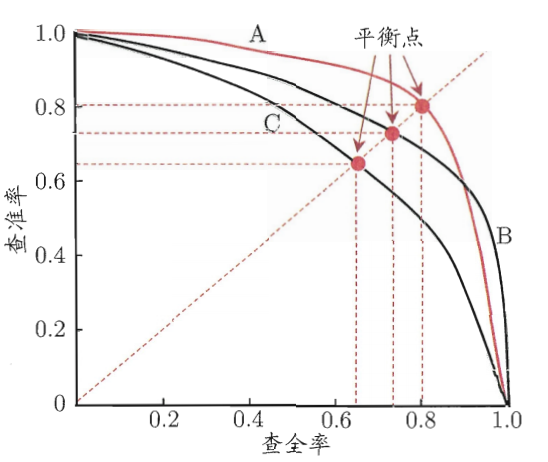
\includegraphics[width=0.6\textwidth]{static/images/P-R曲线图.png}
    \caption{P-R曲线示例}
    \label{fig:pr_curve}
\end{figure}
虽然BEP是查准率=查全率时的点,但在实际应用中,查准率和查全率通常不会相等,因此需要综合考虑两者的平衡。
F1值是查准率和查全率的调和平均数,常用来综合评估分类器的性能:
\begin{align}
    F1=\frac{2 \times P \times R}{P+R} \nonumber \\
    &= \frac{2 \times TP}{\text{样例总数}+TP-TN}
\end{align}
但在实际应用中,查准率和查全率的权衡关系通常需要根据具体任务和数据集来调整。所以F1的一般形式--- $F_\beta$,加权调和平均数能够根据任务需求调整查准率和查全率的权重:
\marginpar{与算术平均数和几何平均数相比,调和平均数更重视较小值}
\begin{equation}
    F_\beta = \frac{(1+\beta^2) \times P \times R}{\beta^2 \times P + R}
\end{equation}

对于有多个二分类混淆矩阵的多分类任务,可以使用宏平均(Macro-Averaging)和微平均(Micro-Averaging)来计算整体的查准率、查全率和F1值。
宏平均是对每个类别单独计算查准率和查全率,然后取平均值:
\begin{align}
    P_{macro} &= \frac{1}{n} \sum_{i=1}^{n} P_i \nonumber \\
    R_{macro} &= \frac{1}{n} \sum_{i=1}^{n} R_i \nonumber \\
    F1_{macro} &= \frac{2 \times P_{macro} \times R_{macro}}{P_{macro} + R_{macro}}
\end{align}

微平均则是将所有类别的TP、FP和FN加总后计算查准率和查全率:
\begin{align}
    P_{micro} &= \frac{\sum_{i=1}^{n} TP_i}{\sum_{i=1}^{n} TP_i + \sum_{i=1}^{n} FP_i} \nonumber \\
    R_{micro} &= \frac{\sum_{i=1}^{n} TP_i}{\sum_{i=1}^{n} TP_i + \sum_{i=1}^{n} FN_i} \nonumber \\
    F1_{micro} &= \frac{2 \times P_{micro} \times R_{micro}}{P_{micro} + R_{micro}}
\end{align}
\subsubsection{ROC曲线与AUC}
ROC曲线(Receiver Operating Characteristic Curve)是评估二分类模型性能的常用工具,通过绘制真正率(TPR)与假正率(FPR)的关系来展示分类器在不同阈值下的表现。
真正率(TPR)也称为查全率(Recall),表示实际正例中被正确预测为正例的比例:
\begin{equation}
    \text{TPR} = \frac{\text{TP}}{\text{TP} + \text{FN}}
\end{equation}
假正率(FPR)表示实际负例中被错误预测为正例的比例:
\begin{equation}
    \text{FPR} = \frac{\text{FP}}{\text{FP} + \text{TN}}    
\end{equation}
ROC曲线通过改变分类阈值,计算不同阈值下的TPR和FPR,从而绘制出一条曲线。理想情况下,ROC曲线应尽可能接近左上角(TPR=1, FPR=0),表示模型能够正确识别所有正例且不误判负例。

AUC(Area Under the Curve)是ROC曲线下的面积,表示模型的整体性能。AUC值介于0和1之间,值越大表示模型性能越好。AUC=0.5表示模型没有区分能力,相当于随机猜测;AUC=1表示完美分类器。

\begin{figure}[H]
    \centering
    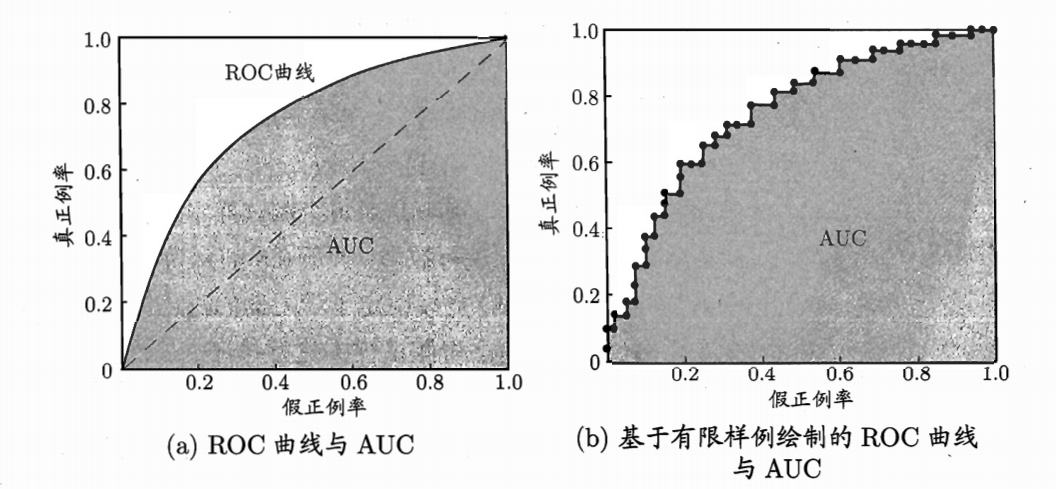
\includegraphics[width=0.6\textwidth]{static/images/ROC曲线与AUC.png}
    \caption{ROC曲线示例}
    \label{fig:roc_curve}
\end{figure}
AUC可以通过计算ROC曲线下的积分来获得,常用的计算方法包括梯形法则和蒙特卡洛积分等。估算公式为:
\begin{equation}
    AUC = \frac{1}{2} \sum_{i=1}^{n-1} (FPR_{i+1} - FPR_i)(TPR_{i+1} + TPR_i)
\end{equation}

形式上看,AUC考虑的是样本预测的排序质量,因此它与排序误差紧密相连,给定$m^+$个正例和$m^-$个反例,令$D^+$和$D^-$分别为正例和反例的样本集

则loss可以表示为:
\begin{equation}
    \ell_{rank} = \frac{1}{m^+ m^-} \sum_{x^+ \in D^+} \sum_{x^- \in D^-}\big( \mathbb{I}(f(x^+) <f(x^-))+\frac{1}{2}\mathbb{I}(f(x^+) = f(x^-))\big)
\end{equation}

容易看出,$\ell_{rank}$对应的是ROC曲线上的面积,故AUC可以表示为:
\begin{equation}
    AUC = 1 - \ell_{rank}
\end{equation}
\subsubsection{代价敏感错误率与代价曲线}
非均等代价: 在某些应用中,不同类型的错误可能具有不同的代价,例如在医疗诊断中,漏诊(假阴性)可能比误诊(假阳性)更严重.
代价敏感错误率: 在这种情况下,需要引入代价敏感错误率来衡量模型的性能,定义为:
\begin{equation}
    E_{f;D;cost} = \frac{1}{m} \big(\sum_{x_i \in D^+} \mathbb{I}(f(x_i) \neq y_i) \cdot cost_{FP} + \sum_{x_i \in D^-} \mathbb{I}(f(x_i) \neq y_i) \cdot cost_{FN}\big)
\end{equation}
其中, $cost_{FP}$和$cost_{FN}$分别表示假正例和假负例的代价.
代价曲线: 代价曲线是代价敏感错误率随分类阈值变化的图形表示,可以帮助选择最优的分类阈值以最小化总代价.
其中,横轴是取值为[0,1]的正例概率代价:
\begin{equation}
    P(+)cost=\frac{p \cdot cost_{FP}}{p \cdot cost_{FP} + (1-p) \cdot cost_{FN}}
\end{equation}
其中,p为正例的概率,纵轴是取值为[0,1]的归一化代价:
\begin{equation}
    cost_{norm}=\frac{FNR \cdot p \cdot cost_{FP} + FPR \cdot (1-p) \cdot cost_{FN}}{p \cdot cost_{FP} + (1-p) \cdot cost_{FN}}
\end{equation}
\begin{figure}[H]
    \centering
    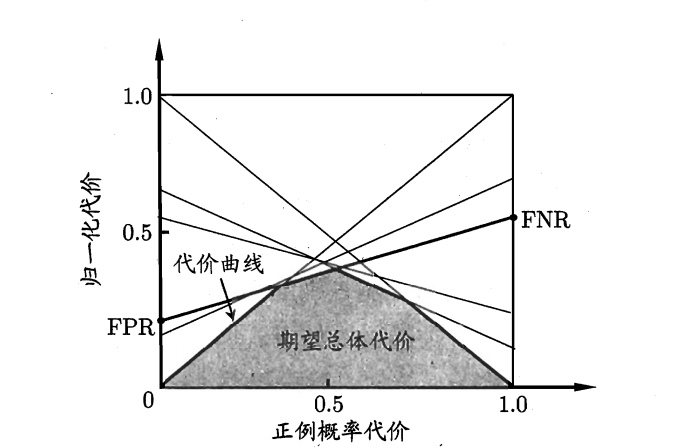
\includegraphics[width=0.6\textwidth]{static/images/代价曲线与期望总体代价.png}
    \caption{代价曲线示例}
    \label{fig:cost_curve}
\end{figure}
\subsection{比较检验}
\subsubsection{假设检验}

